\documentclass[11pt,twocolumn,letterpaper]{article}

\usepackage{cvpr}
\usepackage{times}
\usepackage{epsfig}
\usepackage{graphicx}
\usepackage{amsmath}
\usepackage{amssymb}
\usepackage{mathtools}
\usepackage{array}
\usepackage{multirow}
\usepackage{float}

% Box for the confusion matrix
\newcommand\MyBox[2]{
	\fbox{\lower0.75cm
		\vbox to 1.7cm{\vfil
			\hbox to 1.7cm{\hfil\parbox{1.1cm}{#1#2}\hfil}
			\vfil}%
	}%
}

\usepackage{etoolbox}
\makeatletter
\patchcmd{\@verbatim}
{\verbatim@font}
{\verbatim@font\scriptsize}
{}{}
\makeatother

% Include other packages here, before hyperref.

% If you comment hyperref and then uncomment it, you should delete
% egpaper.aux before re-running latex.  (Or just hit 'q' on the first latex
% run, let it finish, and you should be clear).
\usepackage[breaklinks=true,bookmarks=false]{hyperref}

\cvprfinalcopy % *** Uncomment this line for the final submission

\def\cvprPaperID{****} % *** Enter the CVPR Paper ID here
\def\httilde{\mbox{\tt\raisebox{-.5ex}{\symbol{126}}}}


% Pages are numbered in submission mode, and unnumbered in camera-ready
%\ifcvprfinal\pagestyle{empty}\fi
\setcounter{page}{1}
\begin{document}

%%%%%%%%% TITLE
\title{Assignment 1 \\ COMP SCI 7209 - Introduction to Statistical Machine Learning\\ Support Vector Machine implementation}

\author{Julian Cabezas Pena\\
Student ID: a1785086\\
University of Adelaide, SA 5005 Australia\\
{\tt\small julian.cabezaspena@student.adelaide.edu.au}
% For a paper whose authors are all at the same institution,
% omit the following lines up until the closing ``}''.
% Additional authors and addresses can be added with ``\and'',
% just like the second author.
% To save space, use either the email address or home page, not both
}

\maketitle
%\thispagestyle{empty}


%%%%%%%%% BODY TEXT
\section{Introduction}

In the field of machine learning  and pattern recognition, classification problems are one of the most common tasks. In these kind of problems, an algorithm takes a vector $X$ as input, and assigns it to one or many $K$ discrete classes \cite{Bishop2006}. Considering that the labelled data take values in a discrete set, the input space can be divided in regions that can be labelled according to the classification. Boundaries of these regions can be smooth or rough, depending on the function applied by the algorithm \cite{Hastie2009}. When lineal functions are used to estimate these decision boundaries or surfaces, these algorithms can be labelled as part of the "linear models for classification" family, while data sets whose classes can be separated by lineal functions, are often called to be lineally separable \cite{Bishop2006}.

One of the most common algorithms used in classification problems is the Support Vector Machine (SVM). This supervised classification algorithm was developed by Vapnik \cite{Vapnik1995}, and uses an hyperplane that separates a high dimensional space defined by the input variables into discrete classes. This hyperplane is defined to have the largest possible distances to the closest point of either class \cite{Hastie2009}, thus, maximising the margin ($M$) between two classes. This algorithm can define an hyperplane even when classes overlap (non linearly separable), maximizing the margin but allowing some points to be in the wrong side of the boundary.

The objective of this project is to implement the Support Vector Machine using using convex optimization to solve the primal and dual forms of the algorithm. The implemented methods will be compared with the implementation of the Support Vector Machine Classifier implemented in the commonly used Scikit-learn package, using a simulated dataset.

%-------------------------------------------------------------------------


\section{Methods}

\subsection{Maximal margin classifier}

The margin can be interpreted as the distance of a hyperplane and the closest data points, in the field of machine learning, a hyperplane that can separate two or more classes, maximising the margin (or the distance to the closest points) is called a maximal margin classier (Figure \ref{fig:margin}). This concept is used in many classification algorithms, that seek to maximise this distance. The advantage of this maximal margin classification is that it can produce a great level of generalisation, easily transferring the learning in the training data to the testing data.

\begin{figure}[h]
	\begin{center}
		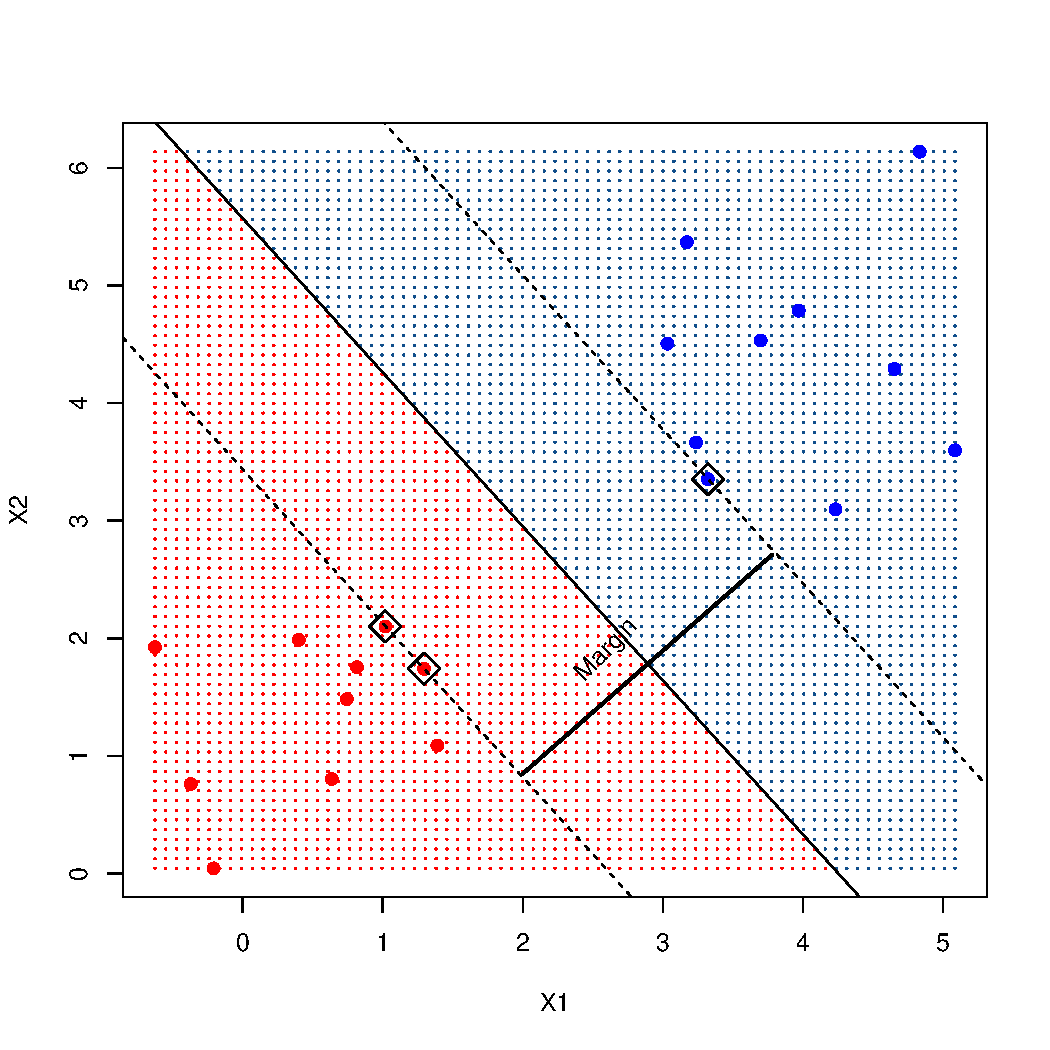
\includegraphics[width=1.0\linewidth]{margin.pdf}
	\end{center}
	\caption{Margin concept - Hard margin SVM (Support vector are inside squares)}
	\label{fig:margin}
\end{figure}

Another big advantage of the maximum margin concept is that it can be easily generalisable to multiple dimensions, allowing to generate multidimensional hyperplanes, the maximum margin classifier can also be applied to transformed data, allowing us to work with kernels \cite{Bishop2006}.

\subsection{Hard Margin SVM}

When implementing the SVM, we can assume we count with $n$ points of data corresponding to pairs of $m$ independent variables $x$ and dependent variable $y$, as $(x_1,y_1), (x_2,y_2), (x_3,y_3) ... (x_n,y_n)$, were $x$ belong to the real realm and $y$ is a vector of true labels coded like ${-1,1}$ (binary class).

The objective of the SVM is to find an hyperplane defined by the coefficients $w$ and the intercept $b$:

\begin{equation}
	f(x) = w^T x + b
\end{equation}

That should give $y_i f(x_i) > 0$ $\forall \: i$, meaning all the samples are well classified, using the sign function as classification rule:

\begin{equation}
	C(x) = sign(w^T x_i + b)
\end{equation}

This constrains are only able to be followed if the dataset is linearly separable, meaning a hyperplane that completely separates the two classes can be found. Hence, the optimization problem is to find the biggest margin $M$ between classes:

\begin{equation}
	max_{w,b} \: M
\end{equation}

\begin{equation}
	subject \:\:to  \:\: y_1(w^T x_i + b) \geq M
\end{equation}

\subsubsection{Primal form}

As the margin can be understood as the distance of the closest points to the hyperplane ($1/||w||$) towards both sides \cite{Hastie2009} (with $||w||$ being the L2 norm), it is possible to conveniently redefine this equation as a minimization problem, as follows:

\begin{equation}
	min_{w,b} \frac{1}{2}||w||^2
\end{equation}

\begin{equation}
	subject \:\:to  \:\: y_i(w^T x_i + b) \geq 1
\end{equation}

This formulation is called the \textbf{primal} form of the problem, and it is considered a convex optimization problem. The Lagrange form (where $\alpha$ are the lagrange multipliers) of this equation can be also written as \cite{Bishop2006}:

\begin{equation}
	L(w,b,\alpha) = \frac{1}{2}||w||^2 - \sum_{i=1}^{n} \alpha_i (y_i(w^T x_i + b) -1) 
\end{equation}

\subsubsection{Dual Form}

If we consider the partial derivatives of w and b in the primal form and set them to be equal to zero, we can get the following conditions:

\begin{equation}
	w = \sum_{i=1}^{n} \alpha_i y_i x_i
\end{equation}

\begin{equation}
	0 = \sum_{i=1}^{n} \alpha_i y_i
\end{equation}

If we eliminate the $b$ and $w$ terms of the primal form equations it is possible to obtain the Lagrangian function \cite{Bishop2006}:

\begin{equation}
	L(\alpha) = \sum_{i=1}^{n} \alpha_i - \frac{1}{2} \sum_{i=1}^{n} \sum_{j=1}^{m} \alpha_i \alpha_j y_i y_j x_i^T x_j
\end{equation}

For computation purposes, it is convenient to express that equation as:

\begin{equation}
	min_{(\alpha)} \frac{1}{2} \sum_{i=1}^{n} \sum_{j=1}^{m} \alpha_i \alpha_j y_i y_j x_i^T x_j - \sum_{i=1}^{n} \alpha_i
\end{equation}

with constrains:

\begin{equation}
	\alpha_i \geq 0  \:\:\: \forall i
\end{equation}

\begin{equation}
	\sum_{i=1}^{n} \alpha_i y_i = 0
\end{equation}

\subsection{Soft Margin SVM}

In real-world data, the data is often not linearly separable, so it is convenient to "allow" the classifier to consider that some points will not be classified correctly, for that, the slack variables $\xi = (\xi_1,\xi_2,\xi_3 ... \xi_n)$ are considered, such that we continue to maximize the margin, but we permit some flexibility, that allows some points to be misclassified, as shown in Figure 2:

\begin{figure}[h]
	\begin{center}
		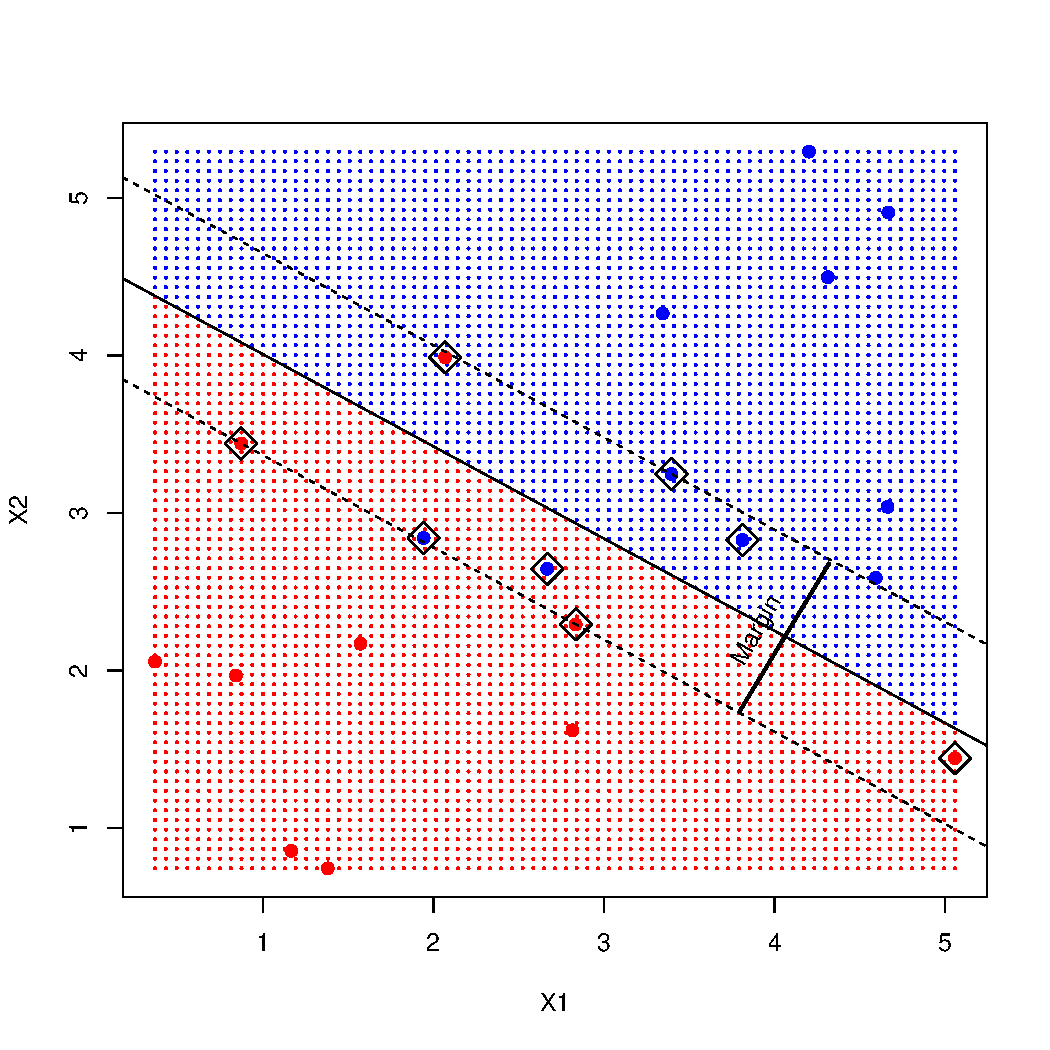
\includegraphics[width=1.0\linewidth]{margin_sf.pdf}
	\end{center}
	\caption{Margin concept - Hard margin SVM (Support vector are inside squares)}
	\label{fig:margin_sf}
\end{figure}


\begin{equation}
	y_i(w^T x_i + b) \geq M - \xi_i 
\end{equation}

\subsubsection{Primal form}

By including this new term, it is possible to write the optimization function as:

\begin{equation}
min \frac{1}{2}||w||^2 + \frac{C}{n} \sum^n_{i=1}\xi_i
\end{equation}

with constrains:

\begin{equation}
y_i(w^T x_i + b) \geq 1 - \xi_i \:\:\:\forall i
\end{equation}

\begin{equation}
	\xi_i  \geq 0 \:\:\: \forall i
\end{equation}

The term C (cost) here is a regularization parameter, that determines the weights of the misclassified samples, with small cost more samples are allowed to be inside de margin boundaries, while a big C will be penalizing those samples harder, this would mean that an infinite C would create a hard margin classifier.

This equation can be also expressed using the Lagrange form 

\begin{multline}
L(w,b,\alpha) = \frac{1}{2}||w||^2 +\frac{C}{n} \sum^n_{i=1}\xi_i \\ \sum_{i=1}^{n} \alpha_i (y_i(w^T x_i + b) - (1 - \xi_i)) - \sum^n_{i=1} \mu_i \xi_i
\end{multline}

\subsubsection{Dual form}

In order to get a more convenient optimizing function, it is possible to set the partial derivatives os $w$, $b$ and $\xi$ to zero \cite{Hastie2009}, getting:

\begin{equation}
	w = \sum_{i=1}^{n} \alpha_i y_i x_i
\end{equation}

\begin{equation}
	0 = \sum_{i=1}^{n} \alpha_i y_i
\end{equation}

\begin{equation}
	\alpha_i = C - \mu_i \:\:\: \forall i
\end{equation}

Obtaining the Lagrange function:

\begin{equation}
	L(\alpha) = \sum_{i=1}^{n} \alpha_i - \frac{1}{2} \sum_{i=1}^{n} \sum_{j=1}^{m} \alpha_i \alpha_j y_i y_j x_i^T x_j
\end{equation}

In order to have a minimizable, it is possible to write the optimization function as:

\begin{equation}
	min_{(\alpha)} \frac{1}{2} \sum_{i=1}^{n} \sum_{j=1}^{m} \alpha_i \alpha_j y_i y_j x_i^T x_j - \sum_{i=1}^{n} \alpha_i
\end{equation}

with constrains (where $\mu$ is a constant)

\begin{equation}
	0 \leq \alpha_i \leq \frac{C}{n}   \:\:\: \forall i
\end{equation}

\begin{equation}
	\sum_{i=1}^{n} \alpha_i y_i = 0
\end{equation}

\subsubsection{The concept of support vectors}

When optimizing these Lagrange functions, typically many of the $\alpha$ values are equal to zero \cite{Hastie2009}, as these points are far away from the separating hyperplane. Thus, the hyperplane is defined by a subset of the the data points, that are called "support vectors", that are shown in Figures 1 and 2.

As the support vectors are close to the hyperplane (Figures 1 and 2), if one of them is removed, the position of the hyperplane would change, thus, if a data point that is not a support vector is removed, the hyperplane would not change. The amount of support vectors that are included in soft margin SVM is influenced by the cost ($C$) parameter, if the C value is bigger, the misclassification would be penalized hardly in the model, making the margin smaller and considering fewer support vectors.

\subsection{Third Party Implementation: \textit{Scikit-learn}}

In order to compare the implemented method with more mainstream application of the Support Vector Machine Classifier, a third party library was used to solve the classification problem. In this case, the Scikit-learn library was chosen due to its wide popularity in the machine learning community.

\textit{Scikit-learn} is a Python library that integrates various tools for statistics and machine learning applications, that include classification, regression, metrics and feature selection, among many others. This library is distributed under a BSD licence and includes compiled code, that makes it very efficient. The library is built using other popular numerical Python libraries, such as \textit{Numpy} and \textit{Scipy} \cite{Pedregosa2011}.

According to the library documentation \footnote{https://scikit-learn.org/stable/modules/svm.html}, the support vector machine algorithms that are implemented in this package can be used for classification, regression and outlier detection. Among the advantages that are listed for this method are its effectiveness in high dimensional spaces, memory efficiency and its capability to use different kernel functions.

The mathematical formulation of the SVM in the scikit-learn package
\footnote{https://scikit-learn.org/stable/modules/svm.html\#svm-mathematical-formulation}
 follows a similar approach to what was previously explained, with the minimization function in the primal form being:

 
 \begin{equation}
 min_ {w, b, \zeta} \frac{1}{2} w^T w + C \sum_{i=1}^{n} \xi_i\\
  \end{equation}
 

 with constrains:
 
 \begin{equation}
 	y_i (w^T \phi (x_i) + b) \geq 1 - \zeta_i
 \end{equation}
 
 \begin{equation}
 	\xi_i  \geq 0 \:\:\: \forall i
 \end{equation}
 
As the SVM implementation of this library can work with several kernel functions. The constraint includes the $\phi$, transformation, that can take the form of a linear, radial, polynomial or sigmoid function. As the focus of this project is to compare this implementation with the primal and dual forms explained above, the function to be used is the linear function, meaning that $w^T \phi (x_i)$ is equal to $w^T x_i$.

Additionally, as in the minimization function $w^T w$ can be interpreted as  $||w||^2$, it is possible to rewrite the equation as 

\begin{equation}
	min \frac{1}{2}||w||^2 + \frac{C}\sum^n_{i=1}\xi_i
\end{equation}

with constrains:

\begin{equation}
	y_i(w^T x_i + b) \geq 1 - \xi_i \:\:\:\forall i
\end{equation}

\begin{equation}
	\xi_i  \geq 0 \:\:\: \forall i
\end{equation}

Thus, the only difference between the implementation described in section 2.2.1 and the one implemented in Scikit-learn is the form of the regularization parameter $C$, that in this case is not divided by the number of samples ($C/n$).  

The optimization problem in this library is solved using the dual form of the problem, that also has the same difference regarding the cost parameter. Given that fact, to compare the two methods, the cost parameter was divided by the number of samples ($C/n$).

\subsection{Train and testing}

\subsubsection{Databases}

The database in which the implemented methods will be tested corresponds to two datasets. In one hand, the train dataset counts with the 8500 records of data and 200 features, with a target variable that contains two classes, that were encoded as ${-1,1}$. Additionally, the test dataset has 1500 samples, and the same amount of features (200). The database is not linearly separable, thus the soft margin implementation of the SVN (both in its primal and dual forms) were used to train the model in the train dataset and get predictions in the test data.

\subsubsection{Cross validation - C Parameter tuning}

As the $C$ (cost) parameter can have a critical importance on the performance of the SVN model, a 5-fold cross validation on the train data was used to select the best C value in $C = (1,10,20,30,40,50,60,70,80,90,100)$. To perform this, the train database was divided into 5 folds (subsets of the database) with equal number of samples, for each value of C that was tested, 4 of these folds were used to train the model, and then this model was used to predict the target feature in the remaining fold, to then calculate the accuracy as:

\begin{equation}
	accuracy = \frac{TP+TN}{TP+FP+TN+FN}
\end{equation}

Where $TP$ is the number of true positive, $TP$: true negative, $FP$: false positives and $FN$: false negatives.

This process was repeated 5 times for each C value, and then the accuracy was averaged. The best C parameter was selected using the maximum value of mean accuracy.

Giving the above mentioned differences in the Scikit-learn $C$ parameter, the cost values that were tested in this case were divided by the number of samples in the model ($C/n$) for comparison purposes.

\subsubsection{Model testing}

Once the C parameter was selected for the primal, dual and Scikit-learn implementation of the SVN, the best C parameter was used to train the model using the complete train dataset, then, this model was used to predict the target variable in the test dataset, measuring the archived accuracy. 

\subsection{Code}

The code to reproduce this project was attached to this report. The primal and dual implementations of the models were programmed in Python 3.7 using the CVXOPT tool for convex optimization, and followed the API directions of this tool for the solving of the problem \footnote{https://cvxopt.org/userguide/coneprog.html}:

\begin{equation}
	min \frac{1}{2} x^TPx + q^T
\end{equation}

subject to 

\begin{equation}
	Gx \leq b
\end{equation}

\begin{equation}
	Ax = b
\end{equation}

Where $x$ corresponds to the values to be optimized, that in the primal form are the vector $[w,b,\xi]$ and in the dual form $[\alpha]$. The matrices P,q,G,b,A and b were constructed to match the dual and primal minimization problems.

As the cross validation to select the optimal C values can take several hours (depending of the computing power of the equipment), the code of the primal and dual implementations (support\_vector\_machine\_primal\_dual.py) was separated into several steps, and as the steps 1 and 2 can take a great amount of time, the software stores the intermediate results into .csv files, that are placed into the "./Cross\_Validation" folder. These results are read if a .csv file is detected in this folder, skipping the cross validation process (steps 3 and 4):

\begin{itemize}
	\item Step 0: Data Input and Preprocessing
	\item Step 1: Cross validation for the tuning of the C-parameter in the primal form of  the SVM
	\item Step 2: Cross validation for the tuning of the C-parameter in the dual form of the SVM
	\item Step 3: Training and testing of the final primal form SVM model
	\item Step 4: Training and testing of the final dual form SVM model
\end{itemize}

On the other hand, the results of the implementation of the SVM using the third party option (Scikit-learn)was placed in a separate Python code (support\_vector\_machine\_sklearn.py), and also stores the results of the cross validation.

The instructions to run the attached codes can be found in Appendix 1, or in the accompanying README.txt file.

\section{Experimental results}

\subsection{C parameter tuning}

The results of the cross-validation process for finding the optimal C value gave the results shown in Figure \ref{fig:cv_cost}. It is important to note that the cost value in the scikit-learn was defined as $C/n$ to make this parameter equivalent to the primal and dual form implementations. As it is possible to notice, the cost values that were tested (from 1 to 100) do not greatly modify the performance of the model, ranging from \%96.84 when $C = 90$ for the Scikit-learn and primal form implementation, and an accuracy of \%97.21 in the best case for all three models when $C = 10$

The behaviour of the three models is very similar, with the primal form and Scikit-learn implementation being almost identical. In all the tested SVM models, the maximum accuracy is archived with the same C value (10, or equivalently in Scikit-learn, 1/n), that what then used to train the final models

\begin{figure}[h]
	\begin{center}
		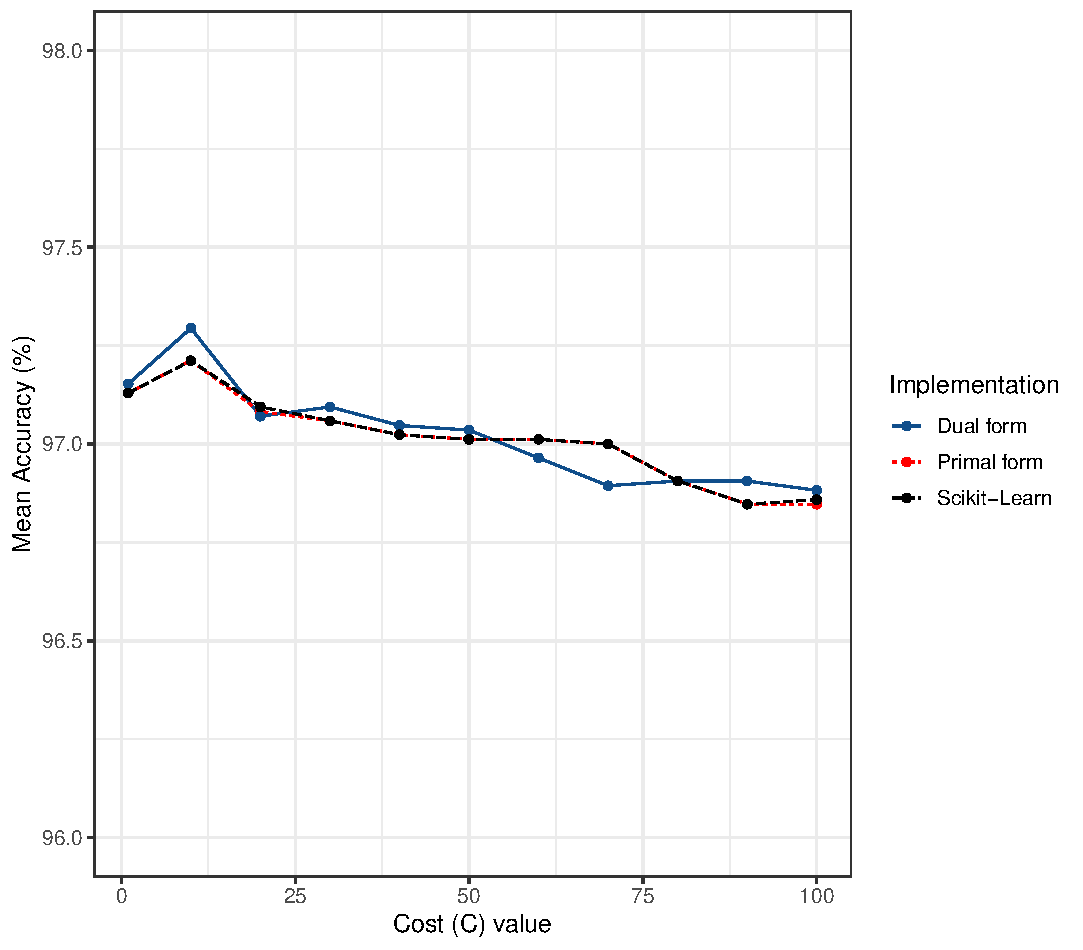
\includegraphics[width=0.9\linewidth]{CV_cost.pdf}
	\end{center}
	\caption{Cost parameter tuning using 5 fold cross validation}
	\label{fig:cv_cost}
\end{figure}


\subsection{Model training}

Using the optimized C parameter, the final models for the implemented SVM forms were trained. The distribution of the weight (w) values (Figure \ref{fig:weights}) shows that 6 out of the 200 variables present larger absolute values, being more influential in the final outcome, as the scaling of the features is relatively similar.

The weights of the three models are similar, with much more noticeable differences in the intercept (b), were the dual form gives $b = 1.1086$, and the primal form and the Scikit-learn implementations yielding $b=1.15601$ (presenting differences after the fourth decimal).

\begin{figure}[h]
	\begin{center}
		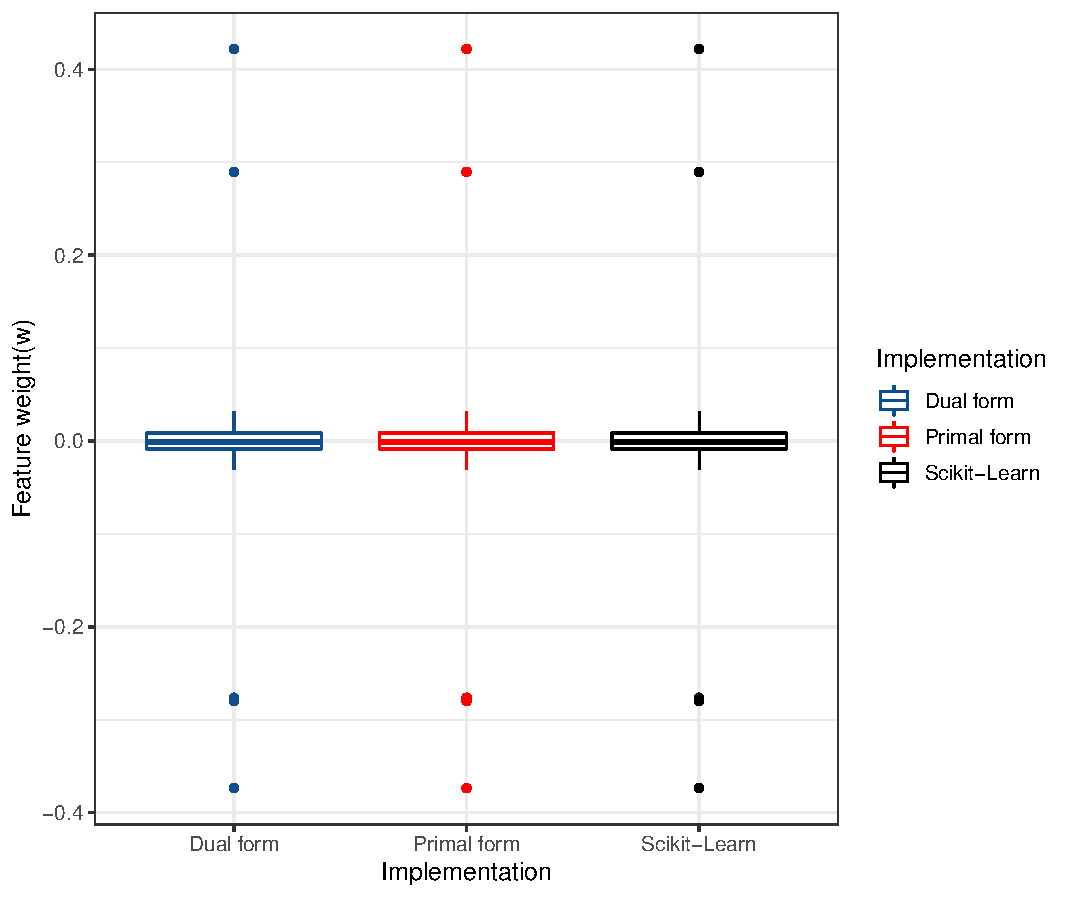
\includegraphics[width=1.0\linewidth]{weights.pdf}
	\end{center}
	\caption{Weights (w) distribution in the models}
	\label{fig:weights}
\end{figure}

\subsection{Training and testing performance}

The results in the training and testing dataset show that the theme models did not show significant overfitting, with the accuracy values in the test data being only slightly smaller than the training accuracy (Table \ref{table:results}), showing the importance of using cross-validation to tune the hyperparameters of the model.

\begin{table}[h]
	\begin{center}
		\begin{tabular}{|p{2cm}|p{1.5cm}|p{1.5cm}|p{1.5cm}|}
			\hline
			SVM Implementation & Best C value & Train accuracy & Test accuracy \\
			\hline\hline
			Primal form & 10 & 0.9764 & 0.9740\\
			Dual form & 10 & 0.9774 & 0.9747\\
			Scikit-learn & 10/8500 & 0.9764 & 0.9740\\
			\hline
		\end{tabular}
	\end{center}
	\caption{SVM implementations train and test accuracy results}
	\label{table:results}
\end{table}

The three models show a test accuracy above 97\%, showing a high predicting performance of the SVM implementations for this database, showing the high performance the SVM can archive, even in non-separable cases.

\section{Conclusion}

This project showed that with enough understanding of the principles and processes behind a maximum margin classifier such as SVM, it is possible to implement an effective classification algorithm using convex optimization libraries. The implemented methods produced almost equal results when compared with third party implementations, showing that it is possible to program complex algorithms that can produce accurate results when the mathematics behind it are well understood.

{\small
\bibliographystyle{ieeetr}
\bibliography{library}
}


\textbf{Appendix 1: Instructions on how to run the attached code:}

This code was tested under a Linux 64 bit OS (Ubuntu 18.04 LTS), using Python 3.7.7

In order to use this code:

1. Install Miniconda or Anaconda
2. Add conda forge to your list of channels

In the terminal run:
\begin{verbatim}
conda config --add channels conda-forge
\end{verbatim}

3. Create a environment using the requirements.yml file included in this .zip:

Open a terminal in the folder were the requirements.yml file is (Assign1-code) and run:

\begin{verbatim}
conda env create -f requirements.yml --name svm-env
\end{verbatim}

4. Make sure the folder structure of the project is as follows

\begin{verbatim}
Assign1-code
├── Input_Data
├── Cross_Validation
├── Results
├── support_vector_machine_primal_dual.py
├── support_vector_machine_sklearn.py
└── ...
\end{verbatim}

If there are csv files in the Cross\_Validation folder the code will read them to avoid the delay of the cross validation and go straight to fitting the models

5.  Run the code in the conda environment: Open a terminal in the Assign1-code folder  and run 
\begin{verbatim}
conda activate svm-env
python support_vector_machine_primal_dual.py
\end{verbatim}

or run the support\_vector\_machine\_primal\_dual.py code in your IDE of preference, (VS Code with the Python extension is recommended), using the root folder of the directory (Assign1-code) as working directory to make the relative paths work.

6. For comparison, run the code of the SVM implementation in Scikit-learn
\begin{verbatim}
python support_vector_machine_sklearn.py
\end{verbatim}
Note: Alternatively, for 2 and 3 you can build your own environment following the package version contained in requirements.yml file

\end{document}



